\documentclass[11pt]{article}
%\renewcommand{\thesection}{\Roman{section}}  %zmiana section na rzymskie
\usepackage[utf8]{inputenc}
\usepackage[OT4]{polski}
\usepackage{tabularx}
\usepackage[margin=60pt]{geometry}
\usepackage{amsmath}
\usepackage{amsfonts}
\usepackage{listings} 
\usepackage[usenames,dvipsnames,table,xcdraw]{xcolor}
\usepackage{array}
\usepackage{sidecap} %do grafik
\usepackage{wrapfig} % j. w.
\usepackage{graphicx} %j.. w.
\usepackage{subfig} %j. w.
\usepackage{booktabs}
\usepackage{longtable}
\usepackage{hyperref}
\usepackage{nicefrac}
\usepackage{multirow}

\begin{document}
%%%%%%%%%%%%%%%%%%%%%%%%%%%%%%%%%%%%%%%%%%%%%%%%%%%%%%%%%%%%%%%%%%%%%%%%%%%%%%%
%%	tabelka
%%%%%%%%%%%%%%%%%%%%%%%%%%%%%%%%%%%%%%%%%%%%%%%%%%%%%%%%%%%%%%%%%%%%%%%%%%%%%%%%

\begin{table}[h!]
	\begin{tabular}{|l|l|l|l|l|l|}	\hline
	\textbf{Laboratorium} & \multirow{2}{*}{ \textbf{\LARGE 4} } & \multicolumn{3}{l|}{ \textbf{Badanie oporu w funkcji temperatury} } &
	\multirow{3}*{\begin{tabular}{l} Zespół w składzie: \\ 1. Paweł Rzońca \\ 2. Paweł Kozioł \\ 3. Agata Sławska\end{tabular}  }\\
	\textbf{Fizyki Ciała Stałego} & & \multicolumn{3}{l|}{\textbf{(metale, półprzewodniki)}} &\\
	\cline{1-5}
	Wydział: \textbf{WFiIS} & \multicolumn{3}{l|}{Kierunek: \textbf{Fizyka Techniczna}} & Rok: \textbf{3} & \\
	\cline{1-5}
	\multicolumn{3}{|l|}{Data wykonania: \textbf{22.10.2015} } & Data oddania: \textbf{5.11.2015} & Ocena: &\\
	\hline
	\end{tabular}
\end{table}

%%%%%%%%%%%%%%%%%%%%%%%%%%%%%%%%%%%%%%%%%%%%%%%%%%%%%%%%%%%%%%%%%%%%%%%%%%%%%%%%


\section*{Aparatura i metodyka}

\textbf{Aparatura}\\
W ćwiczeniu wykorzystaliśmy:\begin{itemize}
\item Multimetry ustawione na wyznaczanie oporu próbek półprzewodników (Ge oraz InSb).
\item Wzorcowy opornik platynowy podłączony do ommomierza.
\item Szklany kriostat, w którym umieszczono próbki półprzewodników.
\item Pompę odpompowującą powietrze z kriostatu.
\item Ciekły azot nalany do termosa, w którym zanurzano kriostat.
\item Grzałka elektryczna, której moc regulowano pokrętłem, a którą używano do ogrzewania kriostatu.
\end{itemize}
\textbf{Przeprowadzenie ćwiczenia} \begin{enumerate}
\item Ustawiono odpowiedni zakres ommomierzy.
\item Odpompowano powietrze z kriostatu.
\item Nalano ciekły azot do termosa i zanurzono w nim kriostat.
\item W czasie oczekiwania na odpowiednie schłodzenie próbki (38 omów na wzorcowym platynowym oporniku) wykreślono krzywą umożliwiajacą zamianę wskazań ommomierza podłaczonego do platyny na temperaturę.
\item Po uzyskaniu odpowiedniej temperatury włączono grzałkę i rozpoczęto pomiary oporu poszczególnych próbek w funkcji oporu platynowego opornika.
\item Wyniki zapisywano do momentu uzyskania oporu platyny rownego 130 omów.
\end{enumerate}

\section*{Opracowanie wyników}
\subsection*{A. Temperaturowa zależność oporu elektrycznego dla wzorcowego termometru platynowego}
W zakresie temperatur od ok. 40 K do 1400 K opór platyny zmienia się liniowo wraz z temperaturą co częściowo przedstawiono na wykresie \ref{w1}.\\
Zależność tą można wyrazić za pomocą wzoru:

\begin{equation}\label{1}
R_{Pt\ 100} (T) = A\cdot T-B
\end{equation}

\begin{figure}[h!]
\centering
\caption{Wykres zależności oporu platyny $R_{Pt\ 100}$ według wzoru \ref{1}, w zakresie temperatur od 100 K do 400 K.}{\label{w1}}
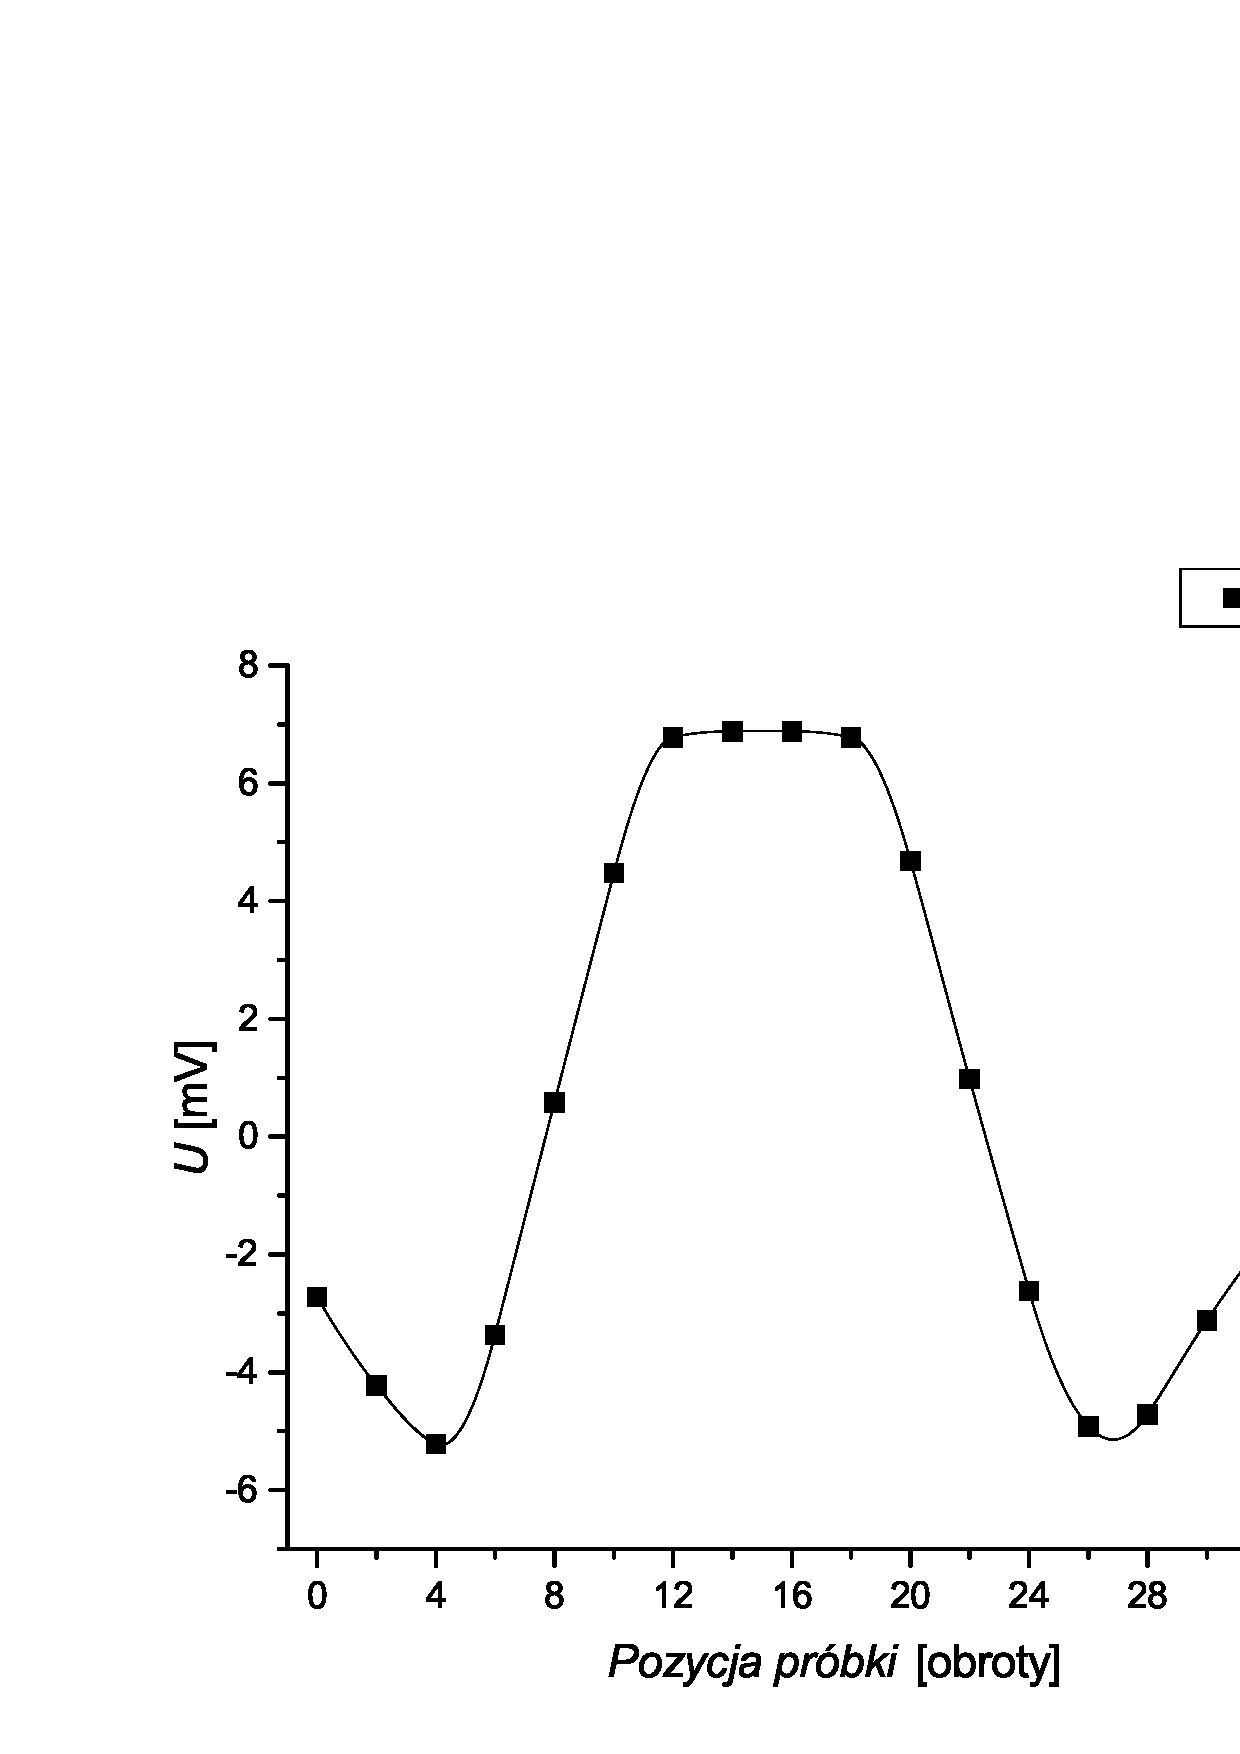
\includegraphics[scale=0.5]{W1.jpg}
\end{figure}


\subsection*{B. Zależność oporu półprzewodników od temperatury, szerokość pasma wzbronionego}
Do poniższej tabeli wpisano wyniki pomiarów dla badanych próbek. Następnie przeliczono opór termometru platynowego na temperaturę w Kelwinach (korzystając 
z charakterystyki termometru platynowego \ref{w1}) i obliczono jej odwrotność. Wyznaczono również przewodność badanych próbek oraz ich logarytm naturalny.
W oparciu o te dane sporządzono wykresy (\ref{w2}, \ref{w3}) przedstawiające zależność logarytmu naturalnego od odwrotności temperatury dla obu badanych materiałów.


\begin{figure}[h!]
\centering
\caption{Wykres logarytmu naturalnego przewodniości od odwrotności temperatury dla $InSb$}{\label{w2}}
\includegraphics[scale=0.5]{W2.jpg}
\end{figure}
\begin{figure}[h!]
\centering
\caption{Wykres logarytmu naturalnego przewodniości od odwrotności temperatury dla termistora}{\label{w3}}
\includegraphics[scale=0.5]{W3.jpg}
\end{figure}


Na każdym z wykresów dopasowano funkcję liniową (dla $InSB$ w dwu zakresach). Na podstawie uzyskanych współczynników 
nachylenia prostych, $A$, korzystając z zależności \ref{2} obliczono szerokości pasma wzbronionego $\Delta E_G $ oraz przerwy
domieszkowej $\Delta E_D$ w $InSb$ oraz $\Delta E_G$ termistora.
\begin{equation}{\label{2}}
A=|\Delta E/k_B|
\end{equation}
gdzie 
$$k_B =  (8,617343 \pm 0,000015 )\cdot 10^{-5} \frac{\mbox{eV}}{\mbox{K}} \qquad [\mbox{Źr. \cite{const}}]$$ 
\\
\\
\\
\\
\\
\\
\\
\\
\\
\\
\\
\section*{Podsumowanie}
Uzyskano następujące wyniki szerokości pasma wzbronionego $\Delta E_G $ oraz przerwy
domieszkowej $\Delta E_D$ w $InSb$ oraz $\Delta E_G$ termistora:
$$
\begin{matrix}
A_{1,InSb} = -3120 \pm 240 [\mbox{K}] & \implies & \Delta E_G = 0,269 \pm 0,020 [\mbox{eV}]\\
A_{2,InSb} = -219 \pm 32 [\mbox{K}] & \implies & \Delta E_D = 0,0189 \pm 0,0028 [\mbox{ev}]\\
A_{term} = -3729\pm 156 [\mbox{K}] & \implies & \Delta E_{term} = 0,321 \pm 0,013 [\mbox{eV}]\\
\end{matrix}
$$
gdzie za współczynnik rozszerzenia niepewności przyjęliśmy $k=2$.
Dla $InSb$ wartości tablicowe $\Delta E_G$  wynosi 
$$\Delta E_G = 0,1725 \ (T=300\mbox{ K}). \quad [\mbox{Źr. \cite{InSb}}] $$
Rozbieżność wyniku jest duża w porównaniu do niepewności wyznaczonej z dopasowania funkcji liniowej. Może to wynikać z niedokładności odczytu oporu, która wynikała przede wszystkim z faktu, iż pomiar nie był wykonywany w stanie ustalonym.   

\begin{thebibliography}{99}
\bibitem{const} \url{http://const.physics.edu.pl/}
\bibitem{InSb} \url{http://www.ioffe.rssi.ru/SVA/NSM/Semicond/InSb/bandstr.html}
\end{thebibliography}



\newpage
\section*{Aneks}

\begin{table}[h!]
\centering
\caption{Wyniki pomiarów oraz obliczeń dla $InSb$ oraz termistora.}
\label{my-label}
\begin{tabular}{|c|c|c|c|c|c|c|c|c|}
\hline
$R_{Pt100}$     & $R_{InSb}$  & $R_{term}$ & $T$    & $1/T$  & $\sigma_{InSb}$     & $\ln (\sigma_{InSb})$    & $\sigma_{term}$      & $\ln (\sigma_{InSb})$    \\ \hline
$[\Omega]$  & $[\mbox{k}\Omega]$ &$[\mbox{k}\Omega]$ & $[\mbox{K}]$ & $[\mbox{K}^{-1}]$ & $[\Omega^{-1}]$ && $[\Omega^{-1}]$ & \\ \hline
32,7           & 78530          & -       & 90,09 & 1,110$\cdot10^{-2}$ &  1,273$\cdot10^{-8}$&-18,179 & -           & -     \\ \hline
35             & 73300          & -       & 96,06 & 1,041$\cdot10^{-2}$ &  1,364$\cdot10^{-8}$&-18,110 & -           & -     \\ \hline
37             & 67100          & -       & 101,25 & 9,876$\cdot10^{-3}$ & 1,490$\cdot10^{-8}$&-18,022 & -           & -     \\ \hline
39             & 60800          & -       & 106,45 & 9,394$\cdot10^{-3}$ & 1,645$\cdot10^{-8}$&-17,923 & -           & -     \\ \hline
41             & 56500          & -       & 111,64 & 8,957$\cdot10^{-3}$ & 1,770$\cdot10^{-8}$&-17,850 & -           & -     \\ \hline
43             & 49800          & -       & 116,84 & 8,558$\cdot10^{-3}$ & 2,008$\cdot10^{-8}$&-17,724 & -           & -     \\ \hline
45             & 44800          & -       & 122,03 & 8,194$\cdot10^{-3}$ & 2,232$\cdot10^{-8}$&-17,618 & -           & -     \\ \hline
47             & 40400          & -       & 127,23 & 7,859$\cdot10^{-3}$ & 2,475$\cdot10^{-8}$&-17,514 & -           & -     \\ \hline
49             & 36600          & -       & 132,42 & 7,551$\cdot10^{-3}$ & 2,732$\cdot10^{-8}$&-17,416 & -           & -     \\ \hline
50             & 34500          & -       & 135,02 & 7,406$\cdot10^{-3}$ & 2,900$\cdot10^{-8}$&-17,356 & -           & -     \\ \hline
54             & 27400          & -       & 145,41 & 6,877$\cdot10^{-3}$ & 3,650$\cdot10^{-8}$&-17,126 & -           & -     \\ \hline
58             & 20700          & -       & 155,80 & 6,418$\cdot10^{-3}$ & 4,831$\cdot10^{-8}$&-16,846 & -           & -     \\ \hline
62             & 14400          & -       & 166,19 & 6,017$\cdot10^{-3}$ & 6,944$\cdot10^{-8}$&-16,483 & -           & -     \\ \hline
66             & 10200          & -       & 176,58 & 5,663$\cdot10^{-3}$ & 9,800$\cdot10^{-8}$&-16,138 & -           & -     \\ \hline
70             & 6700           & -       & 186,97 & 5,348$\cdot10^{-3}$ & 1,493$\cdot10^{-7}$&-15,718 & -           & -     \\ \hline
74             & 4300           & 5800    & 197,36 & 5,066$\cdot10^{-3}$ & 2,326$\cdot10^{-7}$&-15,274 & 1,724$\cdot10^{-7}$ & -15,573 \\ \hline
78             & 2800           & 2900    & 207,75 & 4,813$\cdot10^{-3}$ & 3,571$\cdot10^{-7}$&-14,845 & 3,448$\cdot10^{-7}$ & -14,880 \\ \hline
82             & 1900           & 1550    & 218,14 & 4,584$\cdot10^{-3}$ & 5,263$\cdot10^{-7}$&-14,457 & 6,452$\cdot10^{-7}$ & -14,254 \\ \hline
86             & 1268           & 820     & 228,53 & 4,375$\cdot10^{-3}$ & 7,886$\cdot10^{-7}$&-14,053 & 1,220$\cdot10^{-6}$ & -13,617 \\ \hline
90             & 853            & 420     & 238,92 & 4,185$\cdot10^{-3}$ & 1,172$\cdot10^{-6}$&-13,657 & 2,381$\cdot10^{-6}$ & -12,948 \\ \hline
94             & 525            & 220     & 249,31 & 4,011$\cdot10^{-3}$ & 1,905$\cdot10^{-6}$&-13,171 & 4,545$\cdot10^{-6}$ & -12,301 \\ \hline
98             & 317            & 110     & 259,70 & 3,850$\cdot10^{-3}$ & 3,155$\cdot10^{-6}$&-12,667 & 9,091$\cdot10^{-6}$ & -11,608 \\ \hline
102            & 290            & 65      & 270,09 & 3,702$\cdot10^{-3}$ & 3,448$\cdot10^{-6}$&-12,578 & 1,538$\cdot10^{-5}$ & -11,082 \\ \hline
106            & 210,9          & 35,6    & 280,47 & 3,565$\cdot10^{-3}$ & 4,742$\cdot10^{-6}$&-12,259 & 2,809$\cdot10^{-5}$ & -10,480 \\ \hline
110            & 150,6          & 20,5    & 290,86 & 3,438$\cdot10^{-3}$ & 6,640$\cdot10^{-6}$&-11,922 & 4,878$\cdot10^{-5}$ & -9,928  \\ \hline
114            & 104,4          & 11,98   & 301,25 & 3,319$\cdot10^{-3}$ & 9,579$\cdot10^{-6}$&-11,556 & 8,347$\cdot10^{-5}$ & -9,391  \\ \hline
118            & 76,52          & 7,68    & 311,64 & 3,208$\cdot10^{-3}$ & 1,307$\cdot10^{-5}$&-11,245 & 1,302$\cdot10^{-4}$ & -8,946  \\ \hline
122            & 44,86          & 5,275   & 322,03 & 3,105$\cdot10^{-3}$ & 2,229$\cdot10^{-5}$&-10,711 & 1,896$\cdot10^{-4}$ & -8,571  \\ \hline
126            & 35,323         & 3,575   & 332,42 & 3,008$\cdot10^{-3}$ & 2,831$\cdot10^{-5}$&-10,472 & 2,797$\cdot10^{-4}$ & -8,182  \\ \hline
130            & 27,29          & 2,495   & 342,81 & 2,917$\cdot10^{-3}$ & 3,664$\cdot10^{-5}$&-10,214 & 4,008$\cdot10^{-4}$ & -7,822  \\ \hline
\end{tabular}
\end{table}


\end{document}


